\documentclass[11pt]{article}
\usepackage[utf8]{inputenc}
\usepackage{graphicx}
% \usepackage[figuresleft]{rotating}
\usepackage{pdflscape}
\usepackage{pdfpages}
\usepackage{float}
\usepackage{caption}
\usepackage{subcaption}
\usepackage{longtable}
\graphicspath{ {./} }

\setlength{\parindent}{0em}
\setlength{\parskip}{1em}

% Set up nicer table spacing
\setlength{\arrayrulewidth}{0.5mm}
\setlength{\tabcolsep}{18pt}
\renewcommand{\arraystretch}{1.5}

\usepackage{natbib}
\newcommand*{\urlprefix}{Available from: }
\newcommand*{\urldateprefix}{Accessed }
\bibliographystyle{bathx}

\usepackage{geometry}
\geometry{
  a4paper,
  total={170mm,257mm},
  left=20mm,
  top=20mm,
}
% \geometry{
%   a4paper,
% }
\DeclareCaptionFormat{custom}
{%
    \textbf{#1#2}#3
}
\captionsetup{format=custom}
\captionsetup{width=0.8\textwidth}

\usepackage{csquotes}
\usepackage[hidelinks]{hyperref}
\newcommand{\refreq}[1]{\textbf{\hyperlink{req#1}{UR#1}}}
\newcommand{\definereq}[1]{\hypertarget{req#1}{UR#1}}

% Gantt Chart package
\usepackage{pgfgantt}

\title{An Analysis of Emulation based Fuzz Testing for NRF52 Embedded Software Verification}
\author{Rowan Saunders}
\begin{document}

% A Comparison of Fuzzing-based Verification techniques for the development of NRF52 based embedded systems

% - Emulation: coverage-guided unicorn-afl fuzzing
% - Target: Black-box fuzzing
% - Target: coverage-buided Trace based fuzzing
% - Target/Emulation: Manual Test Scripts

\maketitle

% Title
% - Detailed description of the problem you will seek to address in the project and methodologies (3 pages)
% - Objectives and deliverables for the project (1 - 2 pages)
% - Detailed project plan using appropriate techniques (Gantt Chart) (1-3 pages)
% -- Tasks to undertake, time allocation for the tasks, and dependencies
% - List of required resources to complete the project, their availibility, and alternatives if not available.
% - Attach Ethics Checklist

% TODO:
% - Ethics Checklist (Complete)
% - Read methodology content
% - clarify approach referencing Borsig_2020 esp32 but with nrf52. plus focus on emulation using unicorn.
% - Read Beckmann_2023 (plus 10 other relevent papers)
% - Gantt Chart

% Brief
% - Description of the problem you will seek to address in the project (1 to 2 pages plus references)
% - Identification of the main objectives and deliverables for the project (one page)
% - An outline of the project plan (one page) that identifies the tasks you will undertake and the initial time allocation for those tasks.

% Introduction
% - What is Fuzzing?
% -- Existing Uses: Cybersecurity, systems programs (Browsers)
% -- Comparison with other verification methodologies
% - What is Embedded Software (IOT)?
% - Why Fuzzing for embedded software?
% -- Context for Embedded Software development
% -- Current state of embedded software fuzzing (Yun_2022, Eisele_2022)
% --- Outline from these papers areas to work in (coverage guided fuzzing on target or with emulation)
% -- Challenges with fuzzing embedded systems
% --- Constraints of testing embedded software
% ---- Time
% ---- Money
% -- Cybersecurity risks in IOT
% --- Use of insecure languages with memory errors (C/C++)
% - Introduce NRF52 as common chip for wireless applications
% -- Beckmann_2023 uses simple baremetal NRF52 application (and complex rtos on STM32) using hardware coverage guided testing over SWO interface.



% - Difficulty Testing Embedded Software, IOT, etc.
% - What is Fuzzing? Fuzz testing. Existing Use cases
% - Minimal use of fuzzing for testing IOT/Embedded devices
% - Challenges specific to fuzzing embedded devices
%   - Coverage/Feedback to the Fuzzer
%   - Interfaces/Harnesses
%   - Emulation/Use of hardware

% Identify the Data needed to demonstrate project objectives have been achieved.
% Use a project data table:
% - Objective, How will you prove the objective is achieved, What data is necessarry, How can you obtain the data.
% - | Objective | Proof of achievement? | What data needed? | Method to obtain data? |

% Show a process for fuzz testing the NRF52
% - Develop a Unicorn-AFL based test harness for fuzz testing the example application
% - Develop a Unicorn Emulator for targeted (manual) testing of example application
% - Disscus viability of manual testing vs fuzz testing

% Emulate NRF52 using Unicorn
% Integrate NRF52 Unicorn Emulation with AFL++ unicorn_mode
% Build on work done in https://github.com/befoulad/nrf52_radio_emu (emulating nrf52 to run bare metal radio firmware)

% Maier_Unicorefuzz makes use of unicorn emulation to fuzz test an operating system kernel
% README for afl++ unicorn_mode https://github.com/AFLplusplus/AFLplusplus/blob/stable/unicorn_mode/README.md
% FIRMCORN builds on unicorn to develop their own fuzzer that detects function calls

% - Detailed project plan using appropriate techniques (Gantt Chart) (1-3 pages)
% -- Tasks to undertake, time allocation for the tasks, and dependencies
% - List of required resources to complete the project, their availibility, and alternatives if not available.

% - Pilot study
% -- Simple system (few to no peripherals to model in unicorn)
% -- identify test corpus
% -- identify manual testing method (emulation)
% -- identify manual testing methodd (on-target)
% -- identify black-box testing method

\section{Problem Description} \label{sec:1}

Embedded systems are becoming more prevalent in today's society, due to the
rise of the Internet of Things (IOT) \citep{Abdumohasan_2021}. Embedded
software is often written in low level languages such as C where errors and
security vulnerabilities are easy to introduce \citep{Svoboda_2021}, and have
many many attack surfaces where these mistakes could be exploited
\citep{Abdumohasan_2021}. Furthermore, many embedded systems have stringent
reliability requirements, such as safety critical software in automotive
devices. As such, verification and testing of embedded systems is paramount to
prevent the presence of security exploits and critical bugs in these devices.

In the non-embedded space, many software programs use a methodology called fuzz
testing to automatically verify the software. Google has used fuzzing to great
effect, detecting over 10000 security vulnerabilities in over 1000 open source
projects through its OSS-Fuzz project \citep{Google_2023}. In its most basic
form, fuzz testing, or fuzzing, consists of generating some input test data and
monitoring the response of the software/system under test (SUT) to this input.
If the fuzzer detects the program has crashed, it saves the generated test data
for analysis by an engineer, and mutates the input data in some way to produce
a different result. This brute force approach is known as black-box fuzzing,
and given enough time to execute, will uncover many exploitable bugs with the
system, such as memory leaks, buffer overflows, and off by one errors. Basic
black-box fuzzing on an embedded system will require some fuzzing harness
\citep{Eisele_et_al_2022} and some method of detecting a fault, such as
performing a liveness check \citep{Yun_2022}. Borsig et al. do not consider
black-box fuzzing as a promising methodology for fuzzing an esp32 based IOT
device, and conclude that white-box and grey-box fuzzing techniques are more
capable \citep{Borsig_2020}.

Compared to black-box fuzzing, white-box fuzzing involves targeted test case
generation through static program analysis techniques, generating a test case
to match every statically identified code path. Microsoft have had success
using white-box fuzzing to identify difficult bugs that were missed by
black-box fuzzing \citep{Godefroid_2012}. However, symbolic execution
techniques used in white-box fuzzing can become unfeasably computationally
expensive for larger projects \citep{Krishnamoorthy_2010}.

Grey-box fuzzing is a middle ground between black-box and white-box fuzzing.
Grey-box fuzzing relies on the fuzzer receiving feedback regarding code
coverage for each generated test-case to mutate and generate further test
cases. This approach allows it to find code paths faster than black-box
testing, but without requiring any static code analysis \citep{Yun_2022}.

Grey-box fuzzing of a program can be easily implemented for application (i.e
non-embedded) software using popular fuzzers like AFL. AFL provides a library
that is linked into the program at compile time, along with several sanitisers,
to instrument the program. This allows AFL to receive coverage information from
the running program during fuzzing \citep{AFL_2019}. Embedded systems often run on
constrained environments, where running the fuzzer on the target hardware would
be unfeasible. As such, the fuzzer and the SUT are run in different
environments, and it is difficult to instrument and forward runtime information
for grey-box fuzzing \citep{Muench_2018}.

Attempts to solve this problem focus either on fuzzing a program running on
target hardware, or in an emulated environment \citep{Eisele_et_al_2022}.
Running in an emulated environment allows easy inspection of the SUT by the
fuzzer, and potentially faster running and parallel tests
\citep{Eisele_et_al_2022}. However, emulating embedded systems correctly is a
hard problem, and due to the diversity in operating systems, hardware,
peripherals etc. often means that development effort spent on emulating one
system cannot be easily transferred to another. Attempts have been made to
automate emulator development, such as Clements et al. HALucinator, which
allows Hardware Abstraction Layer (HAL) functions in a compiled binary to be
stubbed and fuzzed \citep{Clements_2021}.
Chen et al. investigate a novel approach to fuzzing Real Time Operating Systems
(RTOS) which involves slicing a single program into its constituent tasks and
fuzzing them separately on an emulator based on the call graph of the program
\citep{Chen_2022}.

Yun et al. note that most embedded systems fuzzers rely on emulation
\citep{Yun_2022}. However, most bugs found through emulation still need to be
validated on hardware, and so being able to run the fuzz tests directly on the
target hardware is preferable \citep{Eisele_et_al_2022}. Several methods have
been discussed to improve instrumentation and feedback from running fuzz tests
on target hardware. Beckmann et al. propose making use of the tracing
facilities on modern Arm Cortex-M microcontrollers to stream coverage
information back to the fuzzer \citep{Beckmann_2023}. Eisele proposes using a
debugger as a method of inspecting the SUT and providing coverage feedback to a
fuzzer \citep{Eisele_2022}.

During the development of an embedded system, engineers often require access to
representative development hardware to effectively design and write software.
Often, waiting for prototype hardware to start software development does not
align with business deadlines. The use of emulators improves enables engineers
to write embedded software without access to development hardware, improving
productivity and reducing development time.

Existing research into embedded systems fuzzing often focuses on its
cybersecurity applications and benefits. However, fuzz testing can also be an
effective method for general verification of software. AdaCore provide a fuzz
testing tool called GNATfuzz, which enables subprogram level fuzz testing as a
supplement to unit testing for Ada and SPARK embedded software
\citep{gnatfuzz}. By isolating subprograms and building isolated fuzz test
executables in a manner similar to a unit testing framework, GNATfuzz removes
the need to be able to run the full program under a fuzzer, and thus the need
for an emulator or target hardware. However, the effectiveness of this approach
is relient on Ada's extended runtime constraint checking when compared to C
\citep{gnatfuzz}. Furthermore, subprogram level fuzzing is less able detect
more complex issues resulting from interactions with hardware peripherals and
state.

While research into the fuzz testing of embedded systems has been increasing
year by year \citep{Yun_2022}, there are few generic solutions
\citep{Eisele_et_al_2022}. The two main challenges to embedded system fuzzing
when compared to desktop or server systems remain the variety in CPU
architectures in embedded systems, and the lack of an operating system such as
linux for bare metal systems \citep{Eisele_et_al_2022}. Currently, the
availability and ease of use of fuzzing tooling for embedded systems does not
match that of desktop applications. However, while much research outlines the
challenges with current embedded systems fuzzing techniques, it is unclear how
these challenges compare with the effort required to verify embedded software
using traditional techniques. In order to prove that embedded fuzz testing is a
viable alternative to existing verification methods, a comparison of the cost
effectiveness of conducting embedded fuzzing with other verification techniques
is required.

The design and implementation of embedded software and its verification is
highly coupled to hardware. The nordic semiconductor NRF52 family of
microcontrollers are a common choice for IOT devices. NRF52s are based on the
ARM Cortex-M architecture, and include embedded radio peripherals, such as
bluetooth low energy and wifi (amongst others). Another common IOT radio
microcontroller is the ESP32, for which Borsig et al. previously developed a
fuzzing framework \citep{Borsig_2020}. Furthermore, Yun suggested the need for
further research into emulation of specific architectures and devices
\citep{Yun_2022}. An NRF52 was used by Beckmann for on-target coverage guided
fuzzing of a bare metal ARM Cortex-M system using instruction tracing over a
single wire output (SWO) interface \citep{Beckmann_2023}. Additionally, Behrang
outlines a method for using the unicorn cpu emulator to execute NRF52 based
bare-metal radio firmware \citep{Behrang_2023}. The desktop fuzzer AFL++
includes an implementation called "unicorn\_mode" which allows the unicorn
engine to be built with AFL++ support \citep{UnicornMode}. Maier develops the
Unicorefuzz framework and presents an example use of AFL++ Unicorn Mode for
fuzzing kernel modules, which have similar challenges to embedded systems
\citep{Maier_2019}.



% Research Question
% 1. Verification of Real Time Embedded Systems through Fuzz Testing: A Case Study
% 1.1 What Embbeded System?
% - Simple IOT data logger
% - Simple Robot with a couple of sensors and an actuator
% - Synth/dsp device?
% 2. Replacing unit tests with fuzz testing: Automated Software Verification of an Embedded System.

\section{Project Objectives and Deliverables} \label{sec:2}
This research project aims to investigate the perceived difficulty of fuzzing
an embedded system with currently available tooling, and make a comparison
between different fuzzing and other verification methods with regards to that
difficulty. The project will outline the procedure for configuring and
executing the different verification methodologies, and gather data about the
effectiveness, time/effort, and reuseability. The objective of the study is to
prove that applying fuzz testing methodologies during embedded systems
development provides a strong benefit, despite any time/effort costs. The
expectation is that fuzz testing may outperform traditional verification
methods with respect to cost, such as manual systems testing, and prove to have
higher reuseability.

To do this, an example bare-metal embedded system will be developed based on
the NRF52 chip, with sufficient features to be representative of a real device.
Test harnesses required for manual and fuzz testing will be developed, and the
time and tasks to produce these will be tracked. The example firmware will then
be tested with each verification method, and the number of errors discovered,
and time taken to discover them, will be recorded. These quantitive data will
be compared and discussed, along with qualititative anecdotal information
regarding challenges encountered with each proposed method.

% The main objective of the study is to measure and compare the
% cost-effectiveness of emulation based coverage guided fuzzing as a verification
% methodology for an IOT bare metal embedded system with other verification
% methodologies, such as manual testing, black-box fuzzing, and on-target
% coverage guided fuzzing.
% Cost-effectiveness will be explored through measuring
% the time and difficulty of implementing and executing each verification
% technique, alongside the quantity and type of errors identified by the method.

To meet this objective, and based on the work outlined in \textit{Section
\ref{sec:1}}, a unicorn based emulator for the example NRF52 based system will
be developed, with test harnesses for fuzzing with AFL++ UnicornMode. Required
NRF52 hardware peripherals will be modeled in the unicorn based emulator.
Manual test scripts derived from software requirements for the embedded system
will be created, and also run on the emulator. Furthermore, a simple black box
fuzzer will be developed to run on the emulator. The core deliverables will be:

\begin{itemize}
\item A literature review outlining and comparing embedded fuzz testing methodologies
\item The design and implementation of an example NRF52 based embedded system
\item A set of system test scripts for manually testing the example system
\item The implementation of a unicorn NRF52 emulator, with appropriate peripherals modeled
\item A set of error reports and bug investigations resulting from testing the example system with a black-box fuzzer on the unicorn emulator
\item A set of error reports and bug investigations resulting from running the test scripts against the example system on the unicorn emulator
\item A set of error reports and bug investigations resulting from testing the example system with unicorn-afl
\item A discussion comparing each emulation based verification methodology, considering cost effectiveness
\end{itemize}

The main objective outlined will be supplemented with additional extension
objectives. One potential extension to the main objective would include an
additional investigation and comparison with hardware based verification
techniques. Coverage guided fuzzing based on Beckmann's tracing based work
\citep{Beckmann_2023} could be implemented, along with developing a test
harness to execute the manual test scripts and apply the black-box fuzzer on
the target hardware. The deliverables for this extended objective would be as follows:

\begin{itemize}
\item The development of test harnesses for on target verification of the embedded system
\item Tooling, Instrumentation and Harnesses required for on target coverage guided fuzzing of the example system
\item A set of error reports and bug investigations resulting from testing the example system with a black-box fuzzer on the target hardware
\item A set of error reports and bug investigations resulting from running the test scripts against the example system on the target hardware
\item A set of error reports and bug investigations resulting from testing the example system with a coverage guided hardware fuzzer
\item A discussion comparing each hardware based verification methodology, considering cost effectiveness
\end{itemize}

An alternative extension objective would be to measure the effect of system
complexity on the cost effectiveness of each verification methodology.
The example system can be updated to use common IOT peripherals, such as wifi
or bluetooth, and model these in the unicorn emulator. The ease of emulating
and fuzzing an embedded system may be correlated with the complexity of that
system, and using a wireless protocol should improve the relevence of the
results of the study to IOT devices. The deliverables for this extended objective would be as follows:

\begin{itemize}
\item The design and implmentation of an expanded NRF52 based embedded system, including the use of a wireless communication peripheral
\item The implementation of a unicorn NRF52 emulator with wireless peripherals modeled
\item A set of expanded system test scripts for manually testing the updated example system
\item A set of error reports and bug investigations resulting from testing the expanded example system with a black-box fuzzer on the unicorn emulator
\item A set of error reports and bug investigations resulting from running the test scripts against the example system on the unicorn emulator
\item A set of error reports and bug investigations resulting from testing the expanded example system with unicorn-afl
\item A discussion comparing each emulation based verification methodology, considering cost effectiveness and software complexity
\end{itemize}


\pagebreak
\section{Project Plan} \label{sec:3}


% - Extensions

% For the project, an Agile approach is suggested, allowing the requirements,
% design, implementation and fuzz testing functionality to be developed
% incrementally. This is especially important as the design and specification of
% the example system is to enable the demonstration of fuzzing of the system.

% The project is split into Epics, each with an estimate to completion in
% terms of (working) days.
% These are specified in \textit{Table \ref{tab:1}}. From these Epics, tasks will
% be identified in an agile manner. It is likely that the set of tasks will
% change through the course of the project.

% \begin{table}[H]
%     \centering
%     \begin{tabular}{| l | c |}
%         \hline
%         Epic Title & Estimate (days) \\
%         \hline
%         Literature Review & 5 \\
%         Study Fuzzing Tools & 3 \\
%         Study Embedded Systems & 2 \\
%         Example System Requirements Engineering & 3 \\
%         Example System Design & 3 \\
%         Example System Implementation & 15 \\
%         Tooling development and integration & 5 \\
%         Instrumenting example system & 5 \\
%         Fuzz testing example system & 10 \\
%         Writing Documentation & 3 \\
%         Writing Final Report & 10 \\
%         \hline
%     \end{tabular}
%     \caption{Initial list of Epics for the Project}
%     \label{tab:1}
% \end{table}

% The total estimate from all the Epics in \textit{Table \ref{tab:1}} above is 64
% days. Given an expected average rate of 8 working days per calendar month, an
% overall estimate of the expected timeline can be calculated at around 8 months.
% Some example task breakdown for some of these Epics is shown below:

% \begin{itemize}
%     \item Example System Requirements Engineering
%         \begin{itemize}
%             \item Develop use cases for the example embedded system
%             \item Develop system requirements for the example embedded system
%             \item Identify requirements for conducting chosen fuzzing methodology
%         \end{itemize}
%     \item Example System Design
%         \begin{itemize}
%             \item Define interfaces to the example embedded system
%             \item Determine hardware platform, such as processor architecture and peripherals
%         \end{itemize}
%     \item Tooling development and integration
%         \begin{itemize}
%             \item Identify potential issues for fuzzer integration
%             \item Develop scripts for running fuzz tests
%             \item Create build system for project
%             \item Development of test harnesses for example system
%         \end{itemize}
%     \item Instrumenting example system
%         \begin{itemize}
%             \item Determine methodology for conducting fuzz tests
%             \item Develop instrumentation for fuzz tests
%         \end{itemize}
% \end{itemize}

\textit{Figure \ref{fig:top}} shows a top level gantt chart for the duration of
the project. The timeframe in \textit{Figure \ref{fig:top}} is scoped in terms
of week increments (i.e. 5 working days each). The expected duration of the
project of 13 working weeks is equivilent to 65 working days. Given an expected
average working rate of 8 working days per calendar month, an overall estimate
of the expected timeline can be calculated at around 8 months. This aligns with
the chosen completion period.

The project will initially begin with an extended literature
review, gathering and investigating more literature and developing on ideas
outlined in \textit{Section \ref{sec:1}}. This will lead into a pilot study,
where a basic version of the study will be completed. A detailed work breakdown
for the pilot study is shown in \textit{Figure \ref{fig:pilot}}.

% TODO explain content of pilot study
The focus of the pilot study will be a comparison of emulation based fuzzing
with manual testing and black box fuzzing techniques. The initial example system will
be a simplistic IOT device, using few hardware peripherals. A serial interface
will be used to communicate to the device, which will be simple to integrate
with the unicorn-afl fuzzer.

The work conducted in the pilot study will then be revised and built upon for a
more indepth extended study. There are several potential avenues for
investigation in the extended study, and the direction taken at this point will
depend on the output of the literature review and pilot study. The extended
study will aim to meet at least one of the extension objectives in
\textit{Section \ref{sec:2}}. Two alternative detailed plans are shown for the
extended study in \textit{Figure \ref{fig:ext1}} and \textit{Figure
\ref{fig:ext2}}.

The extended study detailed in \textit{Figure \ref{fig:ext1}} expands the
firmware developed in the pilot study to use more peripherals. The serial
interface will be modified to use a wireless protocol, such as wifi or
bluetooth, which is more common for IOT devices. Comparing test methodologies
for a simple and a more complex system may also show that cost effectiveness of
a test methodology is a function of cost effectiveness, as well as exploring
the ease of modification and reusability of the emulator based test
techniques.

The extended study detailed in \textit{Figure \ref{fig:ext2}} configures a
suite of hardware based verification techniques with the example system
developed in the pilot study. It is anticipated that tooling and harnesses
developed in the pilot study for emulated black-box and manual testing will be
able to be easily adapted to their hardware based equivilents. As such, the
main focus of this work will be on implementing the coverage guided hardware
fuzzing tooling and instrumentation. Currently, time estimates for these tasks
are somewhat uncertain, and so performing the coverage guided hardware fuzzing
last out of the three techniques will at least allow a comparison with the
hardware based manual and black box fuzzing if the coverage guided fuzzing
cannot be completed in the time frame.

% TODO write about each alternative extension (perhaps in objectives section?):
% - Emulation of Bluetooth system for fuzzing
% - Compare Target hardware fuzz testing with emulation fuzz testing

% TODO: List of required resources to complete the project, their availibility, and alternatives if not available.
The work outlined in this plan can be completed with a linux based computer.
The outlined work can be fully completed with open source tools, and where
tooling is not available, this will be created as part of the study. Running
the fuzz tests may require leaving a computer for an extended period, or may
require access to a computer with more powerful hardware (e.g. more RAM). If
this is the case, a Virtual Private Server (VPS) can be purchased with the
required capability for executing the fuzz tests. Some tasks in the extended
study may require access to an NRF52 development kit. This has already been
procured, as it may also be useful for experimenting with during the pilot study.


% \newgeometry{
%     a3paper,
%    total={170mm,257mm},
%    left=20mm,
%    top=20mm,
% }
\begin{landscape}
% \begin{figure}[tbh]
%     \begin{center}
%         \begin{ganttchart}[%y unit title=0.4cm,
%             % y unit chart=0.5cm,
%             vgrid,hgrid,
%             expand chart=227mm,
%             title label anchor/.style={below=-1.6ex},
%             title left shift=.05,
%             title right shift=.05,
%             title height=1,
%             progress label text={},
%             bar height=0.7,
%             group right shift=0,
%             group top shift=.6,
%             group height=.3
%             ]{1}{12}
%         % \begin{ganttchart}{1}{22}
%             \gantttitle{Working weeks (5 days)}{12} \\
%             \gantttitlelist{1,...,12}{1} \\
%             \ganttbar[name=litrev]{Literature Review}{1}{1} \\
%             \ganttbar[name=ps]{Pilot Study}{2}{6} \\
%             \ganttbar[name=ext]{Target Hardware Extensions}{7}{12} \\
%             \ganttmilestone[name=complete]{Project completed}{12}
%             \ganttlink{litrev}{ps}
%             \ganttlink{ps}{ext}
%             \ganttlink{ps}{complete}
%             \ganttlink{ext}{complete}
%         \end{ganttchart}
%     \end{center}
%     \caption{Top level Gantt Chart}
% \end{figure}

\begin{figure}[tbh]
    \begin{center}
        \begin{ganttchart}[%y unit title=0.4cm,
            % y unit chart=0.5cm,
            vgrid,hgrid,
            expand chart=227mm,
            title label anchor/.style={below=-1.6ex},
            title left shift=.05,
            title right shift=.05,
            title height=1,
            progress label text={},
            bar height=0.7,
            group right shift=0,
            group top shift=.6,
            group height=.3
            ]{1}{13}
        % \begin{ganttchart}{1}{22}
            \gantttitle{Working weeks (5 days)}{13} \\
            \gantttitlelist{1,...,13}{1} \\
            \ganttbar[name=litrev]{Literature Review}{1}{1} \\
            \ganttbar[name=ps]{Pilot Study}{2}{6} \\
            \ganttbar[name=ext]{Extended Study}{7}{11} \\
            \ganttbar[name=ra]{Results Analysis}{12}{12} \\
            \ganttbar[name=writeup]{Writeup}{13}{13} \\
            \ganttmilestone[name=complete]{Project completed}{13}
            \ganttlink{litrev}{ps}
            \ganttlink{ps}{ext}
            \ganttlink{ext}{ra}
            \ganttlink{ra}{writeup}
            \ganttlink{writeup}{complete}
        \end{ganttchart}
    \end{center}
    \caption{Top Level Gantt Chart}
    \label{fig:top}
\end{figure}

\begin{figure}[tbh]
    \begin{center}
        \begin{ganttchart}[%y unit title=0.4cm,
            % y unit chart=0.5cm,
            vgrid,hgrid,
            expand chart=227mm,
            title label anchor/.style={below=-1.6ex},
            title left shift=.05,
            title right shift=.05,
            title height=1,
            progress label text={},
            bar height=0.7,
            group right shift=0,
            group top shift=.6,
            group height=.3
            ]{1}{25}
        % \begin{ganttchart}{1}{22}
            \gantttitle{Working days}{25} \\
            \gantttitlelist{1,...,25}{1} \\
            \ganttgroup[name=ps]{Pilot Study}{1}{25} \\
            \ganttbar[name=psreq]{Document Example System Requirements}{1}{2} \\
            \ganttbar[name=psdev]{Develop Initial Firmware}{3}{6} \\
            \ganttbar[name=psemu]{Develop Initial Unicorn Emulator}{7}{11} \\
            \ganttbar[name=psperiph]{Model basic NRF52 peripherals}{12}{14} \\
            \ganttbar[name=psconfafl]{Configure Unicorn-AFL Fuzzer}{15}{15} \\
            \ganttbar[name=psrunafl]{Run Unicorn-AFL Fuzzer}{16}{16} \\
            \ganttbar[name=psbbemu]{Integrate Black-box fuzzer with Emulator}{17}{18} \\
            \ganttbar[name=psbbrun]{Run Black-box fuzzer}{19}{19} \\
            \ganttbar[name=psmandev]{Write manual test suite}{20}{21} \\
            \ganttbar[name=psmanemu]{Integrate manual tests with Emulator}{22}{22} \\
            \ganttbar[name=psmanrun]{Run manual test suite}{23}{23} \\
            \ganttbar[name=psanal]{Pilot results analysis}{24}{25} \\
            \ganttmilestone[name=pscomplete]{Pilot study completed}{25}
            \ganttlink{psreq}{psdev}
            \ganttlink{psdev}{psemu}
            \ganttlink{psemu}{psperiph}
            \ganttlink{psperiph}{psconfafl}
            \ganttlink{psconfafl}{psrunafl}
            \ganttlink{psperiph}{psbbemu}
            \ganttlink{psbbemu}{psbbrun}
            \ganttlink{psreq}{psmandev}
            \ganttlink{psperiph}{psmanemu}
            \ganttlink{psmandev}{psmanemu}
            \ganttlink{psmanemu}{psmanrun}
            \ganttlink{psrunafl}{psanal}
            \ganttlink{psbbrun}{psanal}
            \ganttlink{psmanrun}{psanal}
            \ganttlink{psanal}{pscomplete}
        \end{ganttchart}
    \end{center}
    \caption{Detail level Gantt Chart for Pilot Study}
    \label{fig:pilot}
\end{figure}

\begin{figure}[tbh]
    \begin{center}
        \begin{ganttchart}[%y unit title=0.4cm,
            % y unit chart=0.5cm,
            vgrid,hgrid,
            expand chart=227mm,
            title label anchor/.style={below=-1.6ex},
            title left shift=.05,
            title right shift=.05,
            title height=1,
            progress label text={},
            bar height=0.7,
            group right shift=0,
            group top shift=.6,
            group height=.3
            ]{1}{25}
        % \begin{ganttchart}{1}{22}
            \gantttitle{Working days}{25} \\
            \gantttitlelist{1,...,25}{1} \\
            \ganttgroup[name=ex]{Extended Study}{1}{25} \\
            \ganttbar[name=exreq]{Document additional requirements}{1}{2} \\
            \ganttbar[name=exdev]{Extended exiting firmware}{3}{7} \\
            \ganttbar[name=exemu]{Adapt Unicorn emulator}{8}{9} \\
            \ganttbar[name=experiph]{Model additional NRF52 peripherals}{10}{15} \\
            \ganttbar[name=exconfafl]{Configure Unicorn-AFL fuzzer}{16}{16} \\
            \ganttbar[name=exrunafl]{Run Unicorn-AFL fuzzer}{17}{17} \\
            \ganttbar[name=exbbemu]{Adapt Black-box fuzzer emulator harnesses}{18}{18} \\
            \ganttbar[name=exbbrun]{Run Black-box fuzzer}{19}{19} \\
            \ganttbar[name=exmandev]{Write additional manual tests}{20}{20} \\
            \ganttbar[name=exmanemu]{Adapt manual test emulator harnesses}{21}{21} \\
            \ganttbar[name=exmanrun]{Run manual test suite}{22}{22} \\
            \ganttbar[name=exanal]{Extended results analysis}{23}{25} \\
            \ganttmilestone[name=excomplete]{Extended study completed}{25}
            \ganttlink{exreq}{exdev}
            \ganttlink{exdev}{exemu}
            \ganttlink{exemu}{experiph}
            \ganttlink{experiph}{exconfafl}
            \ganttlink{exconfafl}{exrunafl}
            \ganttlink{experiph}{exbbemu}
            \ganttlink{exbbemu}{exbbrun}
            \ganttlink{exreq}{exmandev}
            \ganttlink{experiph}{exmanemu}
            \ganttlink{exmandev}{exmanemu}
            \ganttlink{exmanemu}{exmanrun}
            \ganttlink{exrunafl}{exanal}
            \ganttlink{exbbrun}{exanal}
            \ganttlink{exmanrun}{exanal}
            \ganttlink{exanal}{excomplete}
        \end{ganttchart}
    \end{center}
    \caption{Detail level Gantt Chart for Extended Study where the pilot example system is modified to increase system complexity}
    \label{fig:ext1}
\end{figure}

\begin{figure}[tbh]
    \begin{center}
        \begin{ganttchart}[%y unit title=0.4cm,
            % y unit chart=0.5cm,
            vgrid,hgrid,
            expand chart=227mm,
            title label anchor/.style={below=-1.6ex},
            title left shift=.05,
            title right shift=.05,
            title height=1,
            progress label text={},
            bar height=0.7,
            group right shift=0,
            group top shift=.6,
            group height=.3
            ]{1}{25}
        % \begin{ganttchart}{1}{22}
            \gantttitle{Working days}{25} \\
            \gantttitlelist{1,...,25}{1} \\
            \ganttgroup[name=ex]{Extended Study}{1}{25} \\
            \ganttbar[name=exharness]{Develop base hardware test harness}{1}{3} \\
            \ganttbar[name=exmanadapt]{Adapt existing manual test suite for running on hardware}{4}{5} \\
            \ganttbar[name=exmantest]{Run manual test suite on hardware}{6}{6} \\
            \ganttbar[name=exbbadapt]{Configure Black-box fuzzer for running on hardware}{7}{8} \\
            \ganttbar[name=exbbtest]{Run black-box fuzzer on hardware}{9}{9} \\
            \ganttbar[name=excovresearch]{Research hardware coverage-guided fuzzing methodologies}{10}{12} \\
            \ganttbar[name=excovintegrate]{Integrate coverage guided fuzzer with test harnesses}{13}{16} \\
            \ganttbar[name=excovinstrument]{Instrument SUT according to chosen fuzzing methodology}{17}{21} \\
            \ganttbar[name=excovrun]{Run hardware coverage guided fuzzer}{22}{22} \\
            \ganttbar[name=exanal]{Extended results analysis}{23}{25} \\
            \ganttmilestone[name=excomplete]{Extended study completed}{25}

            \ganttlink{exharness}{exmanadapt}
            \ganttlink{exmanadapt}{exmantest}
            \ganttlink{exharness}{exbbadapt}
            \ganttlink{exbbadapt}{exbbtest}
            \ganttlink{excovresearch}{excovintegrate}
            \ganttlink{exharness}{excovintegrate}
            \ganttlink{excovintegrate}{excovinstrument}
            \ganttlink{excovinstrument}{excovrun}
            \ganttlink{exmantest}{exanal}
            \ganttlink{exbbtest}{exanal}
            \ganttlink{excovrun}{exanal}
            \ganttlink{exanal}{excomplete}
        \end{ganttchart}
    \end{center}
    \caption{Detail level Gantt Chart for Extended Study where the pilot example system is tested with additional verification techniques}
    \label{fig:ext2}
\end{figure}
\end{landscape}
% \restoregeometry



\pagebreak
\bibliography{report.bib}
\pagebreak
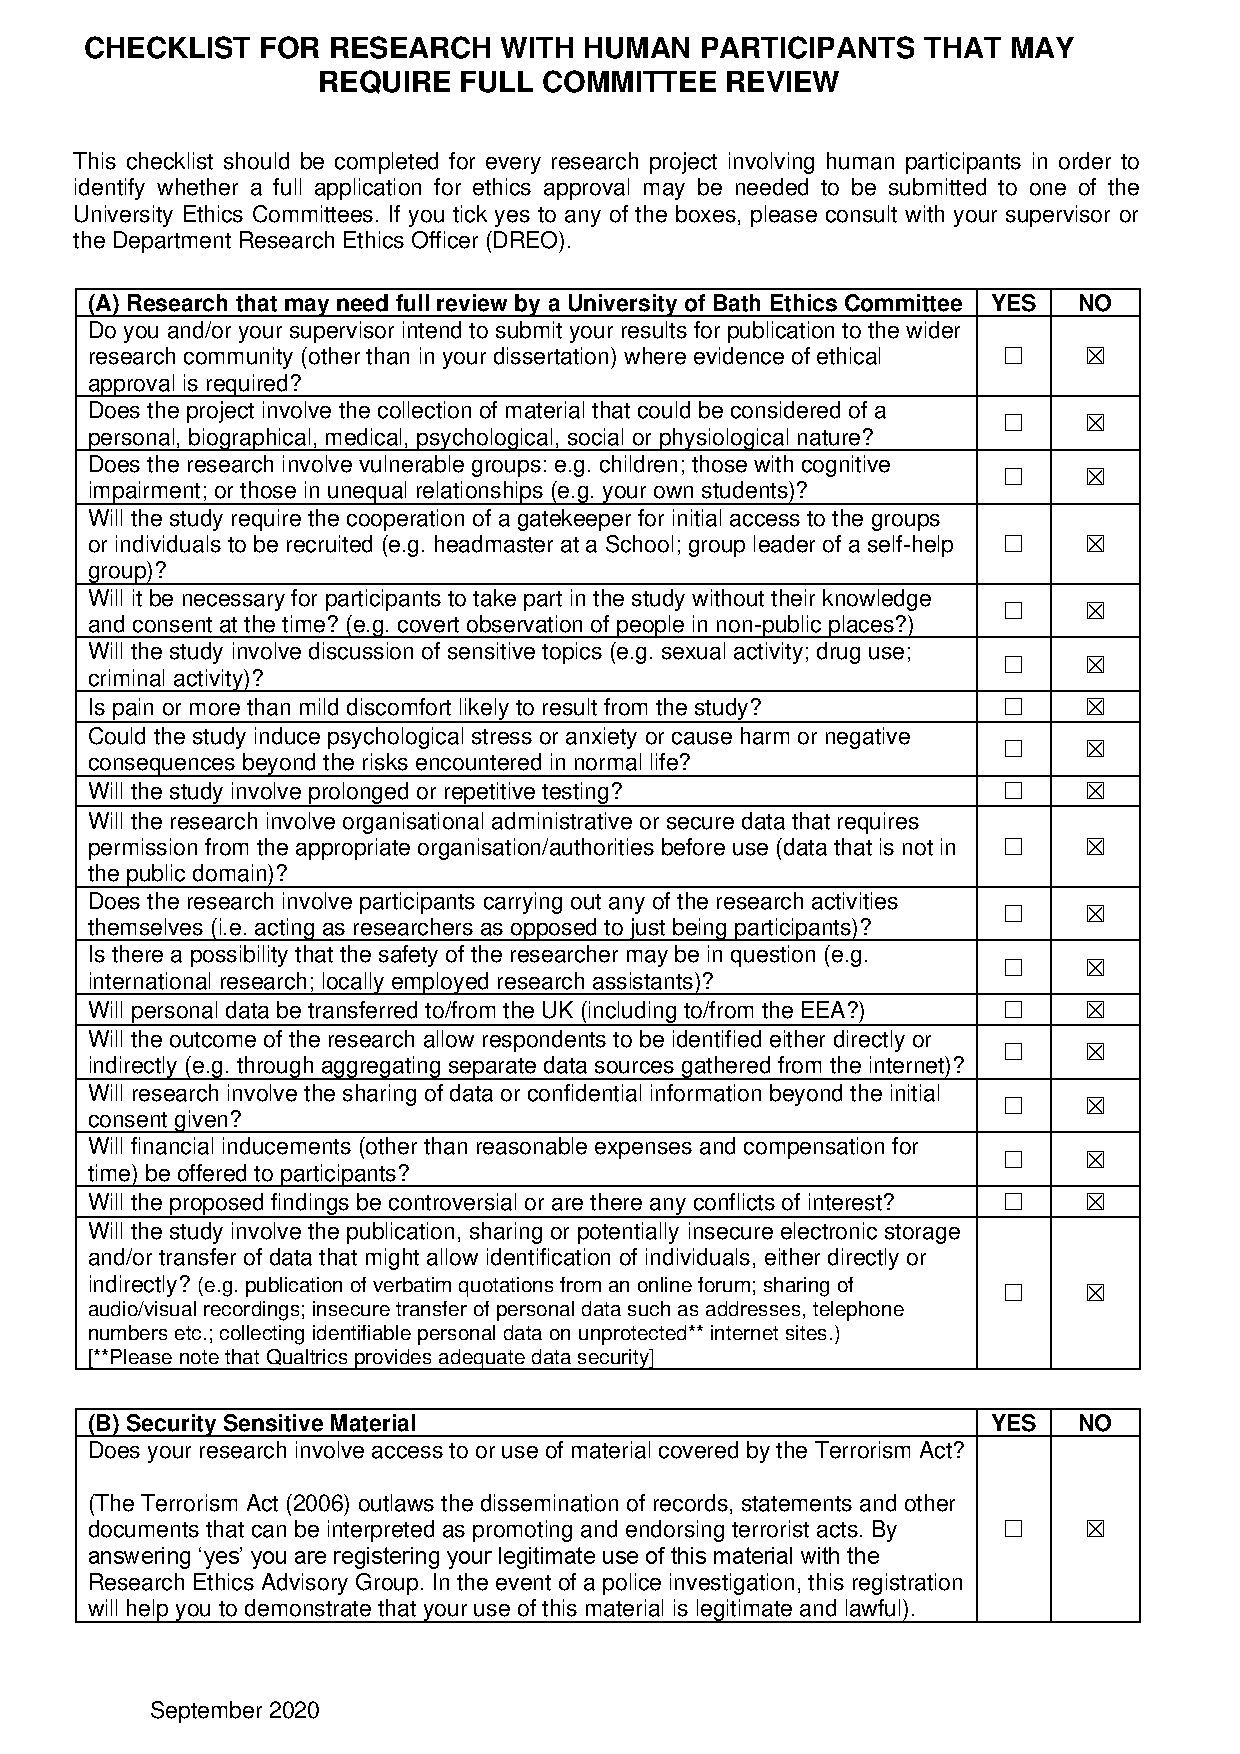
\includepdf[pages=-]{ethics-checklist-1.pdf}

\includepdf[pages=-]{ethics-checklist-2.pdf}



\end{document}
